% =====================================================================
% Seminário — Entropia da fibra do mapa aleatório de Pelikan
% Figuras em figs/, geradas pelo notebook figuras.ipynb
% Parte principal: 14 slides (sem \pause). Depois do "Obrigado": apêndice.
% =====================================================================
\documentclass[11pt,aspectratio=169]{beamer}
\usepackage[utf8]{inputenc}
\usepackage[T1]{fontenc}
\IfFileExists{portuges.ldf}{\usepackage[brazil]{babel}}{\usepackage[english]{babel}}
\IfFileExists{lmodern.sty}{\usepackage{lmodern}}{}
\usepackage{amsmath,amssymb}
\usepackage{booktabs}
\usepackage{tikz}
\usepackage{algpseudocode}
\algrenewcommand\algorithmicfor{\textbf{para}}
\algrenewcommand\algorithmicdo{\textbf{:}}
\algnotext{EndFor}
\algrenewcommand\algorithmicreturn{\textbf{resultado:}}
\algrenewcommand{\algorithmiccomment}[1]{\hfill\textcolor{cinza}{$\triangleright$ #1}}

% ---------- aparência ----------
\usetheme{default}
\setbeamertemplate{navigation symbols}{}
\setbeamertemplate{footline}{\hfill\insertframenumber\hspace{1em}\vspace{0.6em}}
\definecolor{azul}{HTML}{2563EB}
\definecolor{laranja}{HTML}{EA580C}
\definecolor{cinza}{HTML}{6B7280}
\setbeamercolor{frametitle}{fg=azul}
\setbeamercolor{title}{fg=azul}
\setbeamercolor{block title}{bg=azul!15,fg=azul!70!black}
\setbeamercolor{block body}{bg=azul!5}
\setbeamerfont{frametitle}{size=\large,series=\bfseries}
\setbeamertemplate{itemize items}{\textcolor{azul}{\textbullet}}

\newcommand{\hfib}{h_{\mathrm{fib}}}
\newcommand{\lar}[1]{\textcolor{laranja}{#1}}
\newcommand{\cin}[1]{\textcolor{cinza}{#1}}

\title{Entropia da fibra de um sistema aleatório}
\subtitle{Cálculo numérico pelo método de Ulam}
\author{Edeilson Costa de Azevedo Filho}
\institute{ICMC--USP}
\date{}

\begin{document}

% ================================ 1 ==================================
\begin{frame}
  \titlepage
\end{frame}

% ================================ 2 ==================================
\begin{frame}{Setup}
  \vspace{-0.3em}
  \begin{columns}[T]
    \column{0.5\textwidth}
    \begin{block}{Base: o shift}
      \vspace{-0.6em}
      \[
        \Omega=\{0,1\}^{\mathbb N}, \quad
        \sigma(\omega_0\omega_1\omega_2\ldots)=\omega_1\omega_2\ldots
      \]
      \vspace{-1.2em}
      \[
        P_p=\big((1-p)\,\delta_0+p\,\delta_1\big)^{\mathbb N}
      \]
    \end{block}
    \column{0.44\textwidth}
    \begin{block}{Fibra: dois mapas em $[0,1)$}
      \vspace{-0.6em}
      \[
        f_0(x)=\frac x2 \quad \cin{\text{(contrai)}}
      \]
      \vspace{-1.2em}
      \[
        f_1(x)=2x \bmod 1 \quad \cin{\text{(expande)}}
      \]
    \end{block}
  \end{columns}
  \vspace{0.8em}
  \[
    F:\Omega\times[0,1)\to\Omega\times[0,1), \qquad
    F(\omega,x)=\big(\underbrace{\sigma\omega}_{\text{base}},\ \underbrace{f_{\omega_0}(x)}_{\text{fibra}}\big)
  \]
  \vspace{0.3em}
  \begin{center}
    \fcolorbox{laranja}{laranja!6}{\parbox{0.76\textwidth}{\centering
      \textbf{Objetivo:} calcular numericamente $\hfib(p)$ pelo método de Ulam\\
      e entender como ela depende de $p$.}}
  \end{center}
\end{frame}

% ================================ 3 ==================================
\begin{frame}{O que sabemos e o que queremos saber}
  \begin{columns}[T]
    \column{0.48\textwidth}
    \begin{block}{Sabemos}
      \begin{itemize}
        \item $p=1$: só $2x \bmod 1$ \ $\Rightarrow\ \hfib=\log 2$
        \item $p=0$: só contração \ $\Rightarrow\ \hfib=0$
      \end{itemize}
    \end{block}
    \column{0.48\textwidth}
    \begin{block}{Queremos saber}
      \begin{itemize}
        \item o que acontece para $0<p<1$?
        \item é a média $p\log 2$?
        \item Ulam calcula $\hfib$? com que velocidade?
      \end{itemize}
    \end{block}
  \end{columns}
\end{frame}

% ================================ 4 ==================================
\begin{frame}{Exemplo: com $p=0{,}3$ a órbita cola em 0; com $p=0{,}7$ ela passeia}
  \centering
  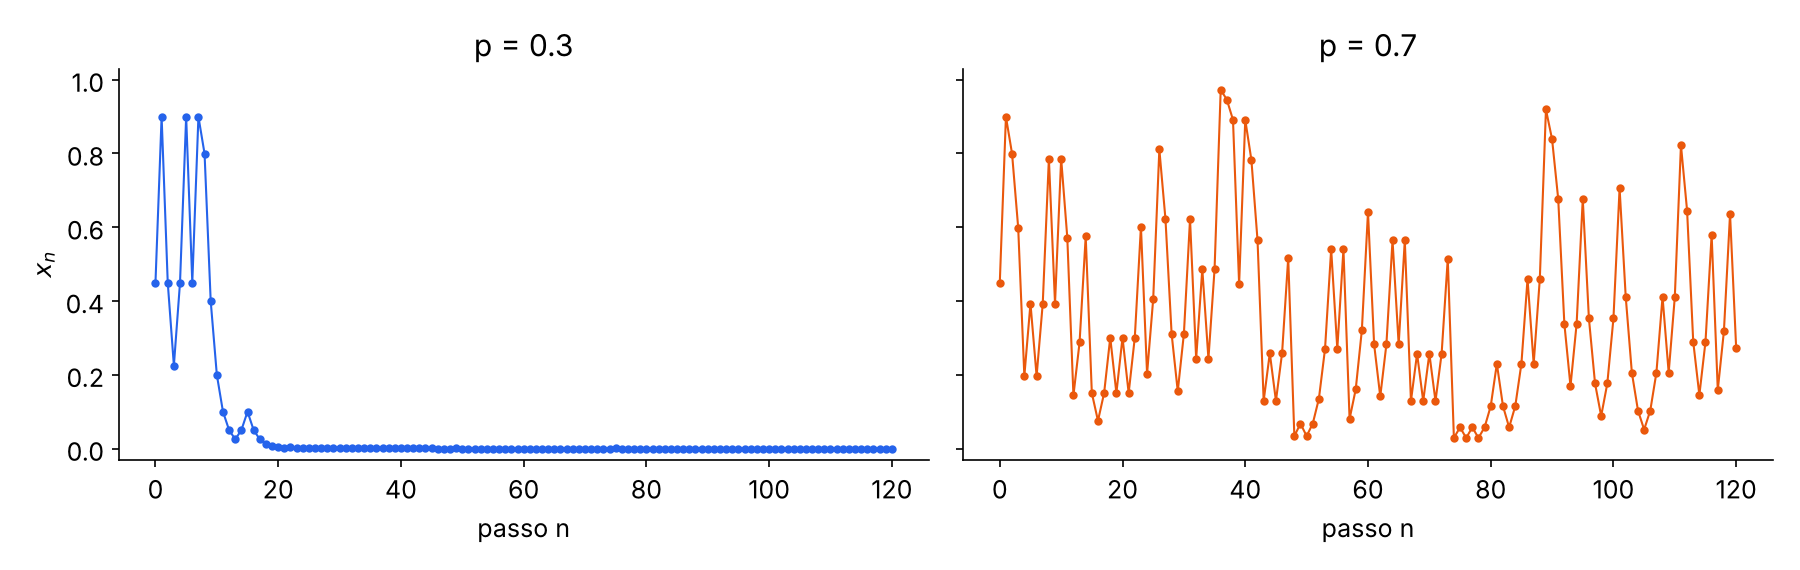
\includegraphics[width=\textwidth]{figs/f1_trajetorias.png}
\end{frame}

% ================================ 5 ==================================
\begin{frame}{Dois pontos quase iguais, mesmos sorteios: se juntam ou se separam?}
  \centering
  $x_0$ e $y_0=x_0+10^{-9}$ recebem \textbf{a mesma} sequência de mapas
  \ \cin{(cada curva = um sorteio)}
  \vspace{0.4em}

  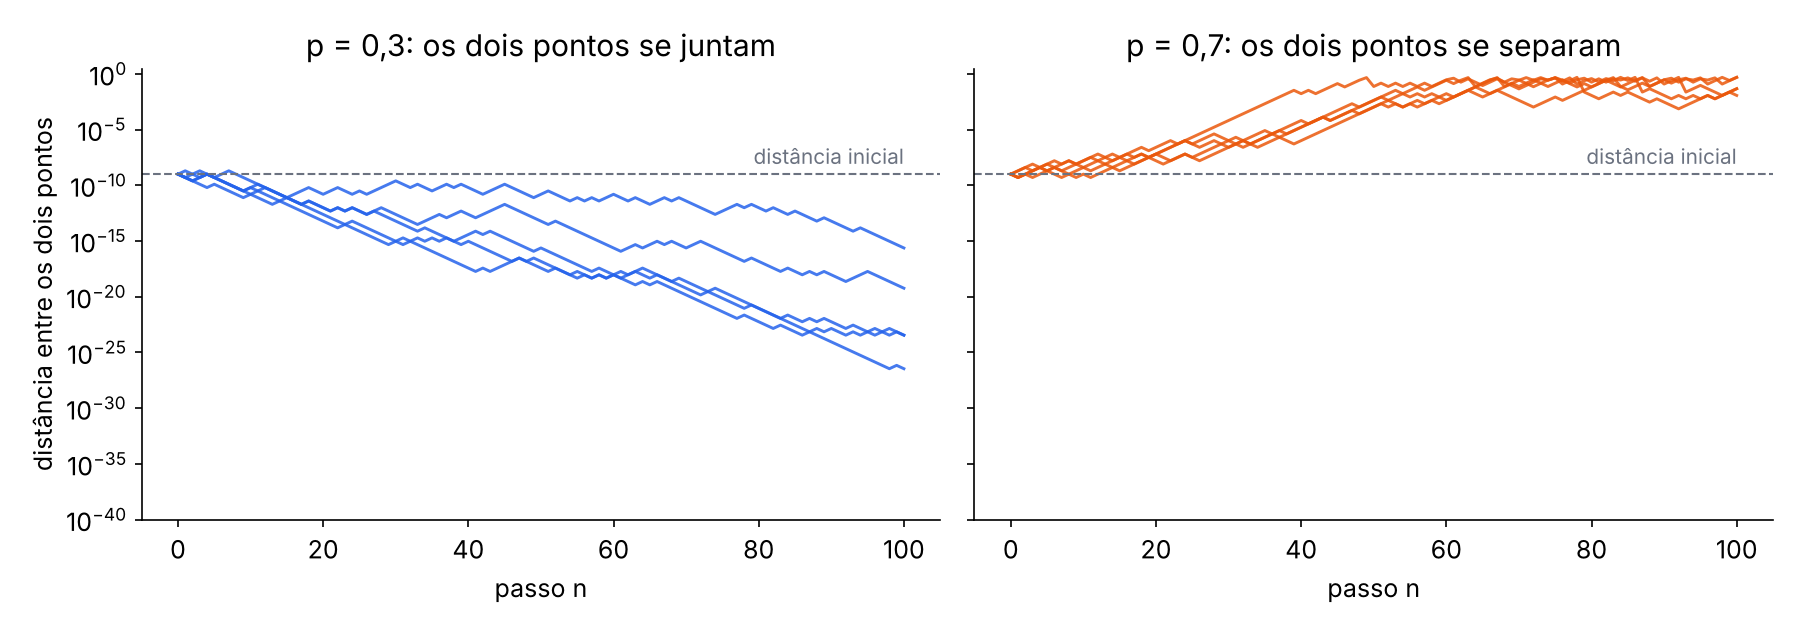
\includegraphics[width=\textwidth]{figs/f2_distancia.png}
\end{frame}

% ================================ 6 ==================================
\begin{frame}{Curiosidade: no computador, a órbita de $2x \bmod 1$ vira 0 em 53 passos}
  \centering
  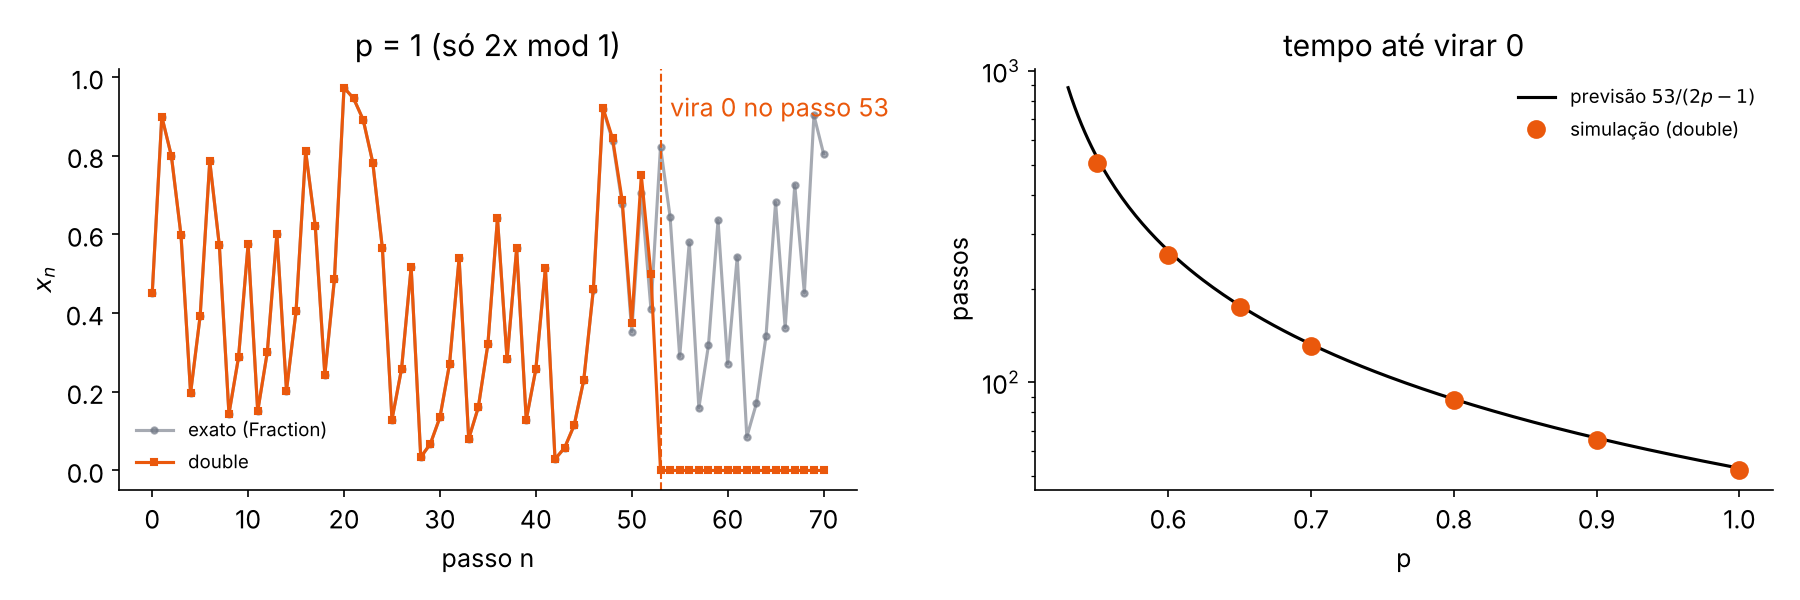
\includegraphics[width=0.92\textwidth]{figs/f3_float.png}
  \vspace{0.2em}

  \small
  \begin{columns}[T]
    \column{0.32\textwidth}
    \textbf{Por quê:} o \texttt{double} guarda 53 dígitos binários; $f_1$ apaga um por passo, $f_0$ não apaga nada.
    \column{0.32\textwidth}
    \textbf{Com sorteios:} morre em $\approx 53/(2p-1)$ passos \\
    \cin{= precisão $\div$ dígitos consumidos por passo}
    \column{0.32\textwidth}
    \textbf{Consequência:} órbitas longas em \texttt{double} são falsas $\Rightarrow$ Ulam usa só $n$ passos por célula.
  \end{columns}
\end{frame}

% ================================ 7 ==================================
\begin{frame}{Método de Ulam: quanto cada célula se espalha?}
  Divida $[0,1)$ em células $I_0, I_1, \dots$ \ e escolha uma palavra $\omega$ (ex.: $\omega = 01$).
  \begin{block}{Matriz de Ulam da palavra $\omega$}
    \vspace{-0.6em}
    \[
      U^{(\omega)}_{ij} \;=\; \frac{\text{comprimento da parte de } I_i \text{ que cai em } I_j}{\text{comprimento de } I_i}
    \]
    \centering \cin{= fração da célula $i$ que termina na célula $j$ depois de aplicar os mapas de $\omega$}
  \end{block}
  \begin{block}{Quão espalhada a célula ficou}
    \vspace{-0.6em}
    \[
      H_i(\omega) = -\sum_j U^{(\omega)}_{ij}\log U^{(\omega)}_{ij}
      \qquad
      \begin{cases}
        \text{cai toda em 1 célula} & \Rightarrow\ H_i=0\\
        \text{metade em cada de 2} & \Rightarrow\ H_i=\log 2
      \end{cases}
    \]
  \end{block}
  \vspace{-0.4em}
  \[
    \hat h_n(p) = \frac1n \sum_{\omega \text{ de tamanho } n} \underbrace{p^{\#1}(1-p)^{\#0}}_{\text{prob. de } \omega}\ \cdot\ \text{média}_i\, H_i(\omega)
  \]
\end{frame}

% ================================ 8 ==================================
\begin{frame}{Pseudocódigo}
  \begin{columns}
    \column{0.9\textwidth}
    \begin{block}{}
      \begin{algorithmic}[1]
        \For{cada palavra $\omega$ de tamanho $n$ \ (ex.: $0110$)}
          \For{cada célula $I_i$}
            \State espalhe muitos pontos dentro de $I_i$
            \State aplique os mapas de $\omega$, um por vez \Comment{0: $x/2$ \quad 1: $2x \bmod 1$}
            \State $U_{ij} \gets$ fração dos pontos que terminaram em $I_j$
            \State $H_i \gets -\sum_j U_{ij}\log U_{ij}$
          \EndFor
          \State $H(\omega) \gets$ média dos $H_i$
        \EndFor
        \State \Return $\hat h_n = \dfrac1n\sum_\omega p^{\#1}(1-p)^{\#0}\, H(\omega)$
      \end{algorithmic}
    \end{block}
  \end{columns}
  \vspace{0.6em}
  \centering \cin{\small entropia de cada palavra primeiro, média depois \quad$\cdot$\quad mais passos $n$ $\Rightarrow$ células menores}
\end{frame}

% ================================ 9 ==================================
\begin{frame}{Exemplo com 4 células: palavras de tamanho $n=1$}
  \centering
  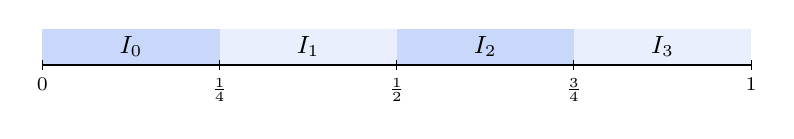
\begin{tikzpicture}[x=9cm,y=1cm]
    \foreach \k/\c in {0/azul!25,1/azul!10,2/azul!25,3/azul!10}
      \fill[\c] (\k/4,0) rectangle ({(\k+1)/4},0.45);
    \draw[thick] (0,0) -- (1,0);
    \foreach \x/\t in {0/0,0.25/\frac14,0.5/\frac12,0.75/\frac34,1/1}
      \draw (\x,-0.06) -- (\x,0.06) node[below=3pt] {\scriptsize $\t$};
    \foreach \k in {0,1,2,3}
      \node at ({(2*\k+1)/8},0.23) {\small $I_{\k}$};
  \end{tikzpicture}
  \vspace{0.2em}

  \begin{columns}[T]
    \column{0.48\textwidth}
    \centering \textbf{$\omega=0$: \ $x\mapsto x/2$}\\[2pt]
    \small $I_0, I_1 \to$ inteiras dentro de $I_0$\\ $I_2, I_3 \to$ inteiras dentro de $I_1$
    \[
      U^{(0)}=\begin{pmatrix}1&0&0&0\\1&0&0&0\\0&1&0&0\\0&1&0&0\end{pmatrix}
      \qquad H_i=\lar{0}
    \]
    \column{0.48\textwidth}
    \centering \textbf{$\omega=1$: \ $x\mapsto 2x \bmod 1$}\\[2pt]
    \small $I_0, I_2 \to \tfrac12$ em $I_0$ e $\tfrac12$ em $I_1$\\ $I_1, I_3 \to \tfrac12$ em $I_2$ e $\tfrac12$ em $I_3$
    \[
      U^{(1)}=\begin{pmatrix}\tfrac12&\tfrac12&0&0\\0&0&\tfrac12&\tfrac12\\\tfrac12&\tfrac12&0&0\\0&0&\tfrac12&\tfrac12\end{pmatrix}
      \qquad H_i=\lar{\log 2}
    \]
  \end{columns}
  \[
    \hat h_1(p)=(1-p)\cdot 0+p\cdot\log 2=\boxed{\,p\log 2\,}
  \]
\end{frame}

% =============================== 9b ==================================
\begin{frame}{Por quê: contrair encolhe a célula, expandir estica e divide em duas}
  \begin{columns}[T]
    \column{0.46\textwidth}
    \centering \textbf{$f_0(x)=x/2$} \ \cin{(tamanho $\times\frac12$)}\\[6pt]
    \renewcommand{\arraystretch}{1.45}
    \small
    \begin{tabular}{cccc}
      \toprule
      célula & imagem & tam. & onde cai\\
      \midrule
      $I_0$ & $[0,\tfrac18)$ & $\tfrac18$ & inteira em $I_0$\\
      $I_1$ & $[\tfrac18,\tfrac14)$ & $\tfrac18$ & inteira em $I_0$\\
      $I_2$ & $[\tfrac14,\tfrac38)$ & $\tfrac18$ & inteira em $I_1$\\
      $I_3$ & $[\tfrac38,\tfrac12)$ & $\tfrac18$ & inteira em $I_1$\\
      \bottomrule
    \end{tabular}\\[6pt]
    \normalsize imagem \textbf{menor} que uma célula\\ $\Rightarrow$ não se espalha: \ $H=\lar{0}$
    \column{0.53\textwidth}
    \centering \textbf{$f_1(x)=2x \bmod 1$} \ \cin{(tamanho $\times 2$)}\\[6pt]
    \renewcommand{\arraystretch}{1.45}
    \small
    \begin{tabular}{cccc}
      \toprule
      célula & imagem & tam. & onde cai\\
      \midrule
      $I_0$ & $[0,\tfrac12)$ & $\tfrac12$ & $\tfrac12$ em $I_0$, $\tfrac12$ em $I_1$\\
      $I_1$ & $[\tfrac12,1)$ & $\tfrac12$ & $\tfrac12$ em $I_2$, $\tfrac12$ em $I_3$\\
      $I_2$ & $[0,\tfrac12)$ & $\tfrac12$ & $\tfrac12$ em $I_0$, $\tfrac12$ em $I_1$\\
      $I_3$ & $[\tfrac12,1)$ & $\tfrac12$ & $\tfrac12$ em $I_2$, $\tfrac12$ em $I_3$\\
      \bottomrule
    \end{tabular}\\[6pt]
    \normalsize imagem do tamanho de \textbf{2 células}\\ $\Rightarrow$ espalha meio a meio: \ $H=\lar{\log 2}$
  \end{columns}
  \vspace{0.6em}
  \centering \footnotesize\cin{$I_0=[0,\tfrac14),\ I_1=[\tfrac14,\tfrac12),\ I_2=[\tfrac12,\tfrac34),\ I_3=[\tfrac34,1)$ \quad$\cdot$\quad cada linha = uma linha de $U^{(\omega)}$}
\end{frame}

% =============================== 10 ==================================
\begin{frame}{Exemplo com 4 células: palavras de tamanho $n=2$}
  \centering \small
  \begin{tabular}{cccc}
    $\omega=00$: \ $x/4$ & $\omega=01$: \ $x$ & $\omega=10$: \ $\tfrac12(2x\bmod1)$ & $\omega=11$: \ $4x\bmod1$\\[4pt]
    $\begin{pmatrix}1&0&0&0\\1&0&0&0\\1&0&0&0\\1&0&0&0\end{pmatrix}$ &
    $\begin{pmatrix}1&0&0&0\\0&1&0&0\\0&0&1&0\\0&0&0&1\end{pmatrix}$ &
    $\begin{pmatrix}1&0&0&0\\0&1&0&0\\1&0&0&0\\0&1&0&0\end{pmatrix}$ &
    $\begin{pmatrix}\tfrac14&\tfrac14&\tfrac14&\tfrac14\\\tfrac14&\tfrac14&\tfrac14&\tfrac14\\\tfrac14&\tfrac14&\tfrac14&\tfrac14\\\tfrac14&\tfrac14&\tfrac14&\tfrac14\end{pmatrix}$\\[14pt]
    $H=0$ & $H=0$ & $H=0$ & $H=\lar{\log 4}$\\
    prob. $(1-p)^2$ & prob. $(1-p)p$ & prob. $p(1-p)$ & prob. $p^2$
  \end{tabular}
  \normalsize
  \[
    \hat h_2(p)=\frac12\Big[(1-p)^2\cdot 0+2p(1-p)\cdot 0+p^2\cdot\log 4\Big]=\boxed{\,p^2\log 2\,}
  \]
  \cin{$01$ e $10$: uma contração desfaz uma expansão $\Rightarrow$ nada se espalha.}
\end{frame}

% =============================== 10b =================================
\begin{frame}{Generalizando: só o saldo positivo conta}
  Palavra com $j$ uns e $n-j$ zeros \ $\Rightarrow$ \ inclinação $2^{S}$, \ $S=j-(n-j)=2j-n$.
  \vspace{0.6em}
  \begin{columns}[T]
    \column{0.48\textwidth}
    \centering \textbf{$S>0$}\\
    cada célula se espalha igualmente\\ por $2^{S}$ células\\[3pt]
    $H=S\log 2$
    \column{0.48\textwidth}
    \centering \textbf{$S\le 0$}\\
    cada célula cai\\ dentro de uma só\\[3pt]
    $H=0$
  \end{columns}
  \vspace{0.6em}
  \begin{block}{}
    \vspace{-0.8em}
    \[
      \hat h_n(p)=\frac{\log 2}{n}\sum_{j=0}^{n}\binom nj p^j(1-p)^{n-j}\,(2j-n)^+
      \ \xrightarrow[n\to\infty]{}\ \lar{(2p-1)^+\log 2}
    \]
  \end{block}
  \centering
  \cin{\small Neste exemplo ``controlado'' há fórmula fechada e o limite é a entropia exata da fibra.\\
  Em geral não há: aí só resta calcular $\hat h_n$ numericamente.}
\end{frame}

% =============================== 10c =================================
\begin{frame}{Para todo $p$, $\hat h_n$ se aproxima do valor exato quando $n$ cresce}
  \centering
  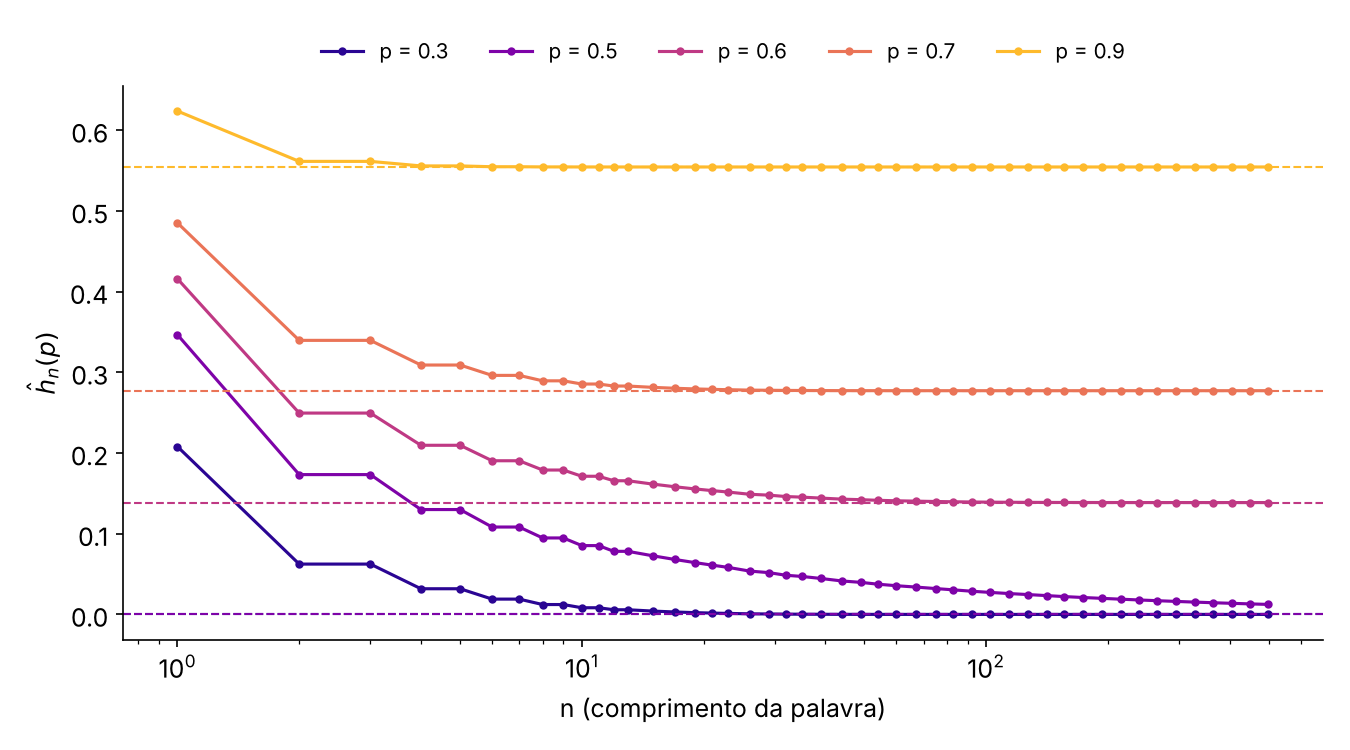
\includegraphics[width=0.85\textwidth]{figs/f9_convergencia_p.png}\\
  \small \cin{tracejado: valor exato $(2p-1)^+\log 2$ \quad$\cdot$\quad $p=0{,}5$ é o mais lento}
\end{frame}

% =============================== 11 ==================================
\begin{frame}{Resultado: Ulam converge para $\hfib(p)=(2p-1)^+\log 2$}
  \begin{columns}
    \column{0.64\textwidth}
    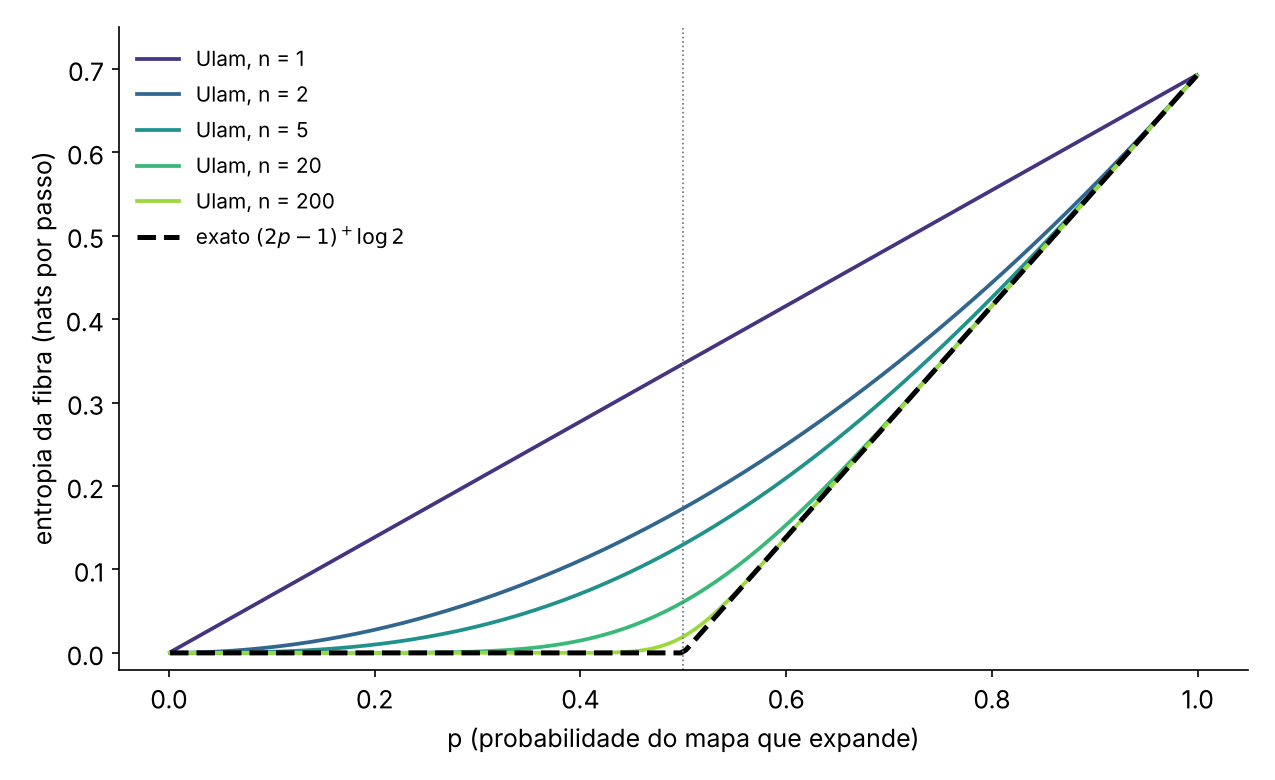
\includegraphics[width=\textwidth]{figs/f7_principal.png}
    \column{0.34\textwidth}
    \begin{itemize}
      \item zero até $p=\tfrac12$
      \vspace{0.4em}
      \item $n=1$: média ingênua $p\log 2$
      \vspace{0.4em}
      \item $n$ cresce $\Rightarrow$ curva exata
    \end{itemize}
  \end{columns}
\end{frame}

% =============================== 13 ==================================
\begin{frame}{Conclusões}
  \vspace{0.5em}
  \Large
  \begin{itemize}
    \item $\hfib(p)=(2p-1)^+\log 2$: \ zero até $p=\tfrac12$
    \vspace{0.6em}
    \item só o \lar{saldo positivo} entre expansão e contração gera entropia
    \vspace{0.6em}
    \item Ulam reproduz o valor exato, \\ mas converge devagar perto de $p=\tfrac12$
  \end{itemize}
\end{frame}

% =============================== 14 ==================================
\begin{frame}
  \centering \Huge \textcolor{azul}{Obrigado!}
\end{frame}

% =====================================================================
%                     APÊNDICE (slides opcionais)
% =====================================================================
\appendix

\begin{frame}{Apêndice: cada recorde do passeio revela um dígito novo}
  \centering
  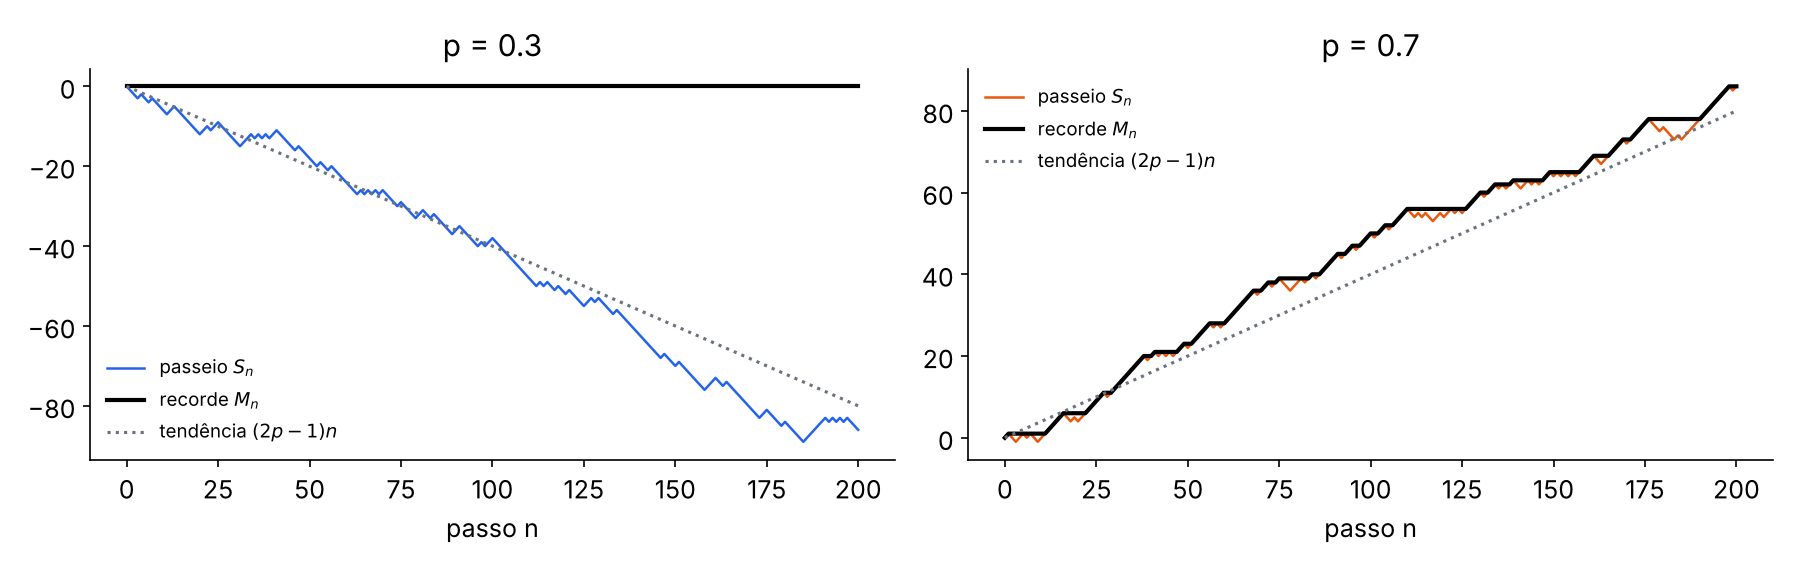
\includegraphics[width=0.95\textwidth]{figs/f4_passeio.png}
  \[
    S_n=\sum_{k<n}(2\omega_k-1),\qquad M_n=\max_{k\le n}S_k,\qquad \frac{M_n}{n}\to(2p-1)^+
  \]
\end{frame}

\begin{frame}{Apêndice: a medida estacionária muda em $p=\tfrac12$}
  \centering
  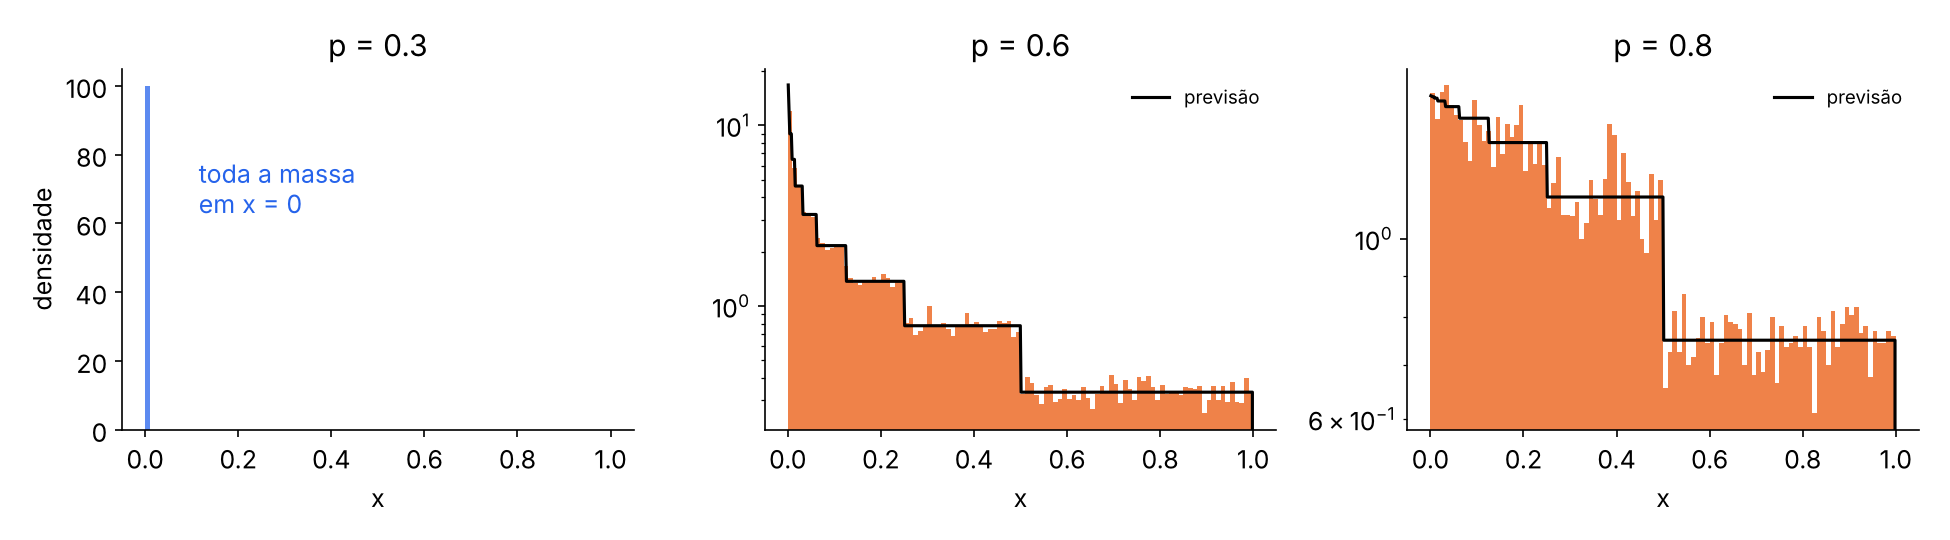
\includegraphics[width=\textwidth]{figs/f5_medida.png}
  \[
    p\le\tfrac12:\ \mu_p=\delta_0 \qquad\qquad p>\tfrac12:\ \text{medida espalhada (Pelikan)}
  \]
  \cin{\small curva preta: $x=2^{-L}U$, $L$ geométrico de razão $\tfrac{1-p}{p}$ (conferir)}
\end{frame}

\begin{frame}{Apêndice: definição da entropia da fibra}
  \[
    \hfib(\mu_p,\mathcal Q)=\lim_{n\to\infty}\frac1n\int_\Omega
    H_{\mu_p}\Big(\bigvee_{k=0}^{n-1}(f^k_\omega)^{-1}\mathcal Q\Big)\,dP_p(\omega),
    \qquad
    \hfib(\mu_p)=\lim_{L\to\infty}\hfib(\mu_p,\mathcal D_L)
  \]
  \[
    \mu_p=(1-p)\,(f_0)_*\mu_p+p\,(f_1)_*\mu_p \quad \text{(estacionária)}
  \]
\end{frame}

\begin{frame}{Apêndice: cuidados numéricos}
  \begin{itemize}
    \item \textbf{Malha cresce com $n$} ($K\ge n$): com $K$ fixo, $H_i\le K\log 2$ e $\hat h_n\to 0$.
    \item \textbf{Composição inteira}: matriz de $f^n_\omega$, não produto de matrizes de um passo.
    \item \textbf{Entropia por palavra, média depois}: a moeda é conhecida.
    \item \textbf{Ponto flutuante}: trajetórias com frações exatas; medida via $x_n=2^{-L}U$.
  \end{itemize}
\end{frame}

\begin{frame}{Apêndice: base, fibra e entropia total}
  \[
    h_{\text{base}}=H(p)=-p\log p-(1-p)\log(1-p)
  \]
  \[
    h_{\text{total}}=H(p)+\hfib(p) \qquad \text{(Abramov--Rokhlin \cin{--- confirmar})}
  \]
\end{frame}

\begin{frame}{Referências}
  \small
  \begin{itemize}
    \item Nota \emph{Ulam entropy} (Graciela).
    \item G. Froyland, \emph{Ulam's method for random interval maps}, Nonlinearity 12 (1999).
    \item C. Monthus, \emph{Explicit dynamical properties of the Pelikan random map}, J. Stat. Mech. (2025).
    \item G. Froyland, O. Junge, G. Ochs, Physica D 154 (2001).
  \end{itemize}
\end{frame}

\end{document}
